In this chapter, we present our reference FPGA application.
We also evaluate the performance of the reference FPGA implementation using the same experimental setup used in chapter \ref{chapter:cpu}.

\section{FPGA implementation} \label{section:reference_fpga}

We have chosen Xilinx's Vitis platform as it seems to be the most popular platform currently \cite{noauthor_vitis_nodate}.
The Vitis platform allows us to write a host program that runs on the CPU that communicates, using OpenCL bindings, with a kernel that runs on the FPGA.
Both the host program and the FPGA kernel are discussed in the following section.

\subsection{Host program} \label{section:fpga_host}

The host program is implemented using the C++ language.
OpenCL is used in the host program to instruct and communicate with the FPGA kernel.
It further uses our FM-index C library from chapter \ref{chapter:cpu} to load an FM-index file from disk into memory.

The steps performed by the host program can be seen in the following timeline:

\begin{enumerate}
  \item Load kernel from disk and program the FPGA
  \item Load FM-index and experiment data from disk
  \item Enqueue OpenCL commands:
  \begin{enumerate}
    \item Migrate experiment data and FM-index data structures to FPGA
    \item Execute FPGA kernel
    \item Migrate result data from FPGA to host program
  \end{enumerate}
  \item Wait until all commands are handled and terminate
\end{enumerate}

Note that enqueuing the OpenCL commands does not block the CPU.
Therefore we must wait until OpenCL is done handling the commands, and the data is migrated to the host.

\subsection{FPGA kernel} \label{section:fpga_kernel}

The FPGA kernel receives a list of patterns, for which it must find the positions in the original text using the FM-index.
These positions are saved in a buffer and sent to the host program when the kernel is done executing.

The FPGA kernel is programmed as an OpenCL kernel and presented in listing \ref{listing:fpga_kernel}.
As can be seen, the kernel is nearly identical to the string search algorithm presented in chapter \ref{chapter:cpu}.
Only minimal changes are made that are required for OpenCL to function.

First of all, the \cinline{reqd_work_group_size} attribute is used to specify how much of the input the kernel can process.
However, we don't use this feature here and we simply set the attribute to all ones.

Next, all input buffers to the kernel have the \cinline{__global} attribute.
This tells the compiler these buffers are located in the global memory on the FPGA.

Lastly, the resulting positions are saved in the global \cinline{out} buffer.
The amount of matches is also saved in this buffer, so we can more easily verify the result on the host.

\begin{listing}[H]
\begin{minted}{c}
kernel __attribute__((reqd_work_group_size(1, 1, 1)))
void fmindex(__global char *bwt,
             __global char *alphabet,
             __global unsigned *ranks,
             __global unsigned *sa,
             __global unsigned *ranges,
             __global char *patterns,
             __global unsigned long *out,
             size_t bwt_sz, size_t alphabet_sz, unsigned pattern_count,
             unsigned pattern_sz, unsigned out_sz) {
  for (unsigned i = 0; i < pattern_count; ++i) {
    int p_idx = pattern_sz - 1;
    char c = patterns[i * pattern_sz + p_idx];
    unsigned start = ranges[2 * string_index(alphabet, c)];
    unsigned end = ranges[2 * string_index(alphabet, c) + 1];

    p_idx -= 1;
    while (p_idx >= 0 && end > 1) {
      c = patterns[i * pattern_sz + p_idx];
      unsigned range_start = ranges[2 * string_index(alphabet, c)];
      int alphabet_idx = string_index(alphabet, c);
      start = range_start + ranks[alphabet_sz * (start - 1) + alphabet_idx];
      end = range_start + ranks[alphabet_sz * (end - 1) + alphabet_idx];
      p_idx -= 1;
    }

    unsigned long match_count = end - start;
    out[i * out_sz] = match_count; // Save match count
    for (unsigned j = 0; j < match_count; ++j)
      out[i * out_sz + j + 1] = sa[start + j]; // Save match position
  }
}
\end{minted}
\caption{The OpenCL Kernel for the reference FPGA application.}
\label{listing:fpga_kernel}
\end{listing}

\section{Empirical evaluation} \label{section:empiric_eval_fpga}

The same experimental setup is used to evaluate our reference FPGA application as for the reference CPU application in section \ref{section:experiment_setup}.
We use timing and energy measurements generated by Vitis \footnote{Thanks Tristaan Laan for the data extraction script}.

\section{Results} \label{section:results_fpga}

In figure \ref{fig:throughput_fpga} the throughput (in patterns matched per second) is shown for the reference FPGA application.
In general, we see that each figure resembles the CPU throughput as shown in section \ref{section:results_cpu}.
The throughput of the \textit{dna} and \textit{proteins} corpora is best, with 30 and 25 thousand top throughput respectively.
The \textit{dblp.xml} corpus only reaches a top throughput of barely 3000 patterns matched per second.

\begin{figure}[H]
\centering
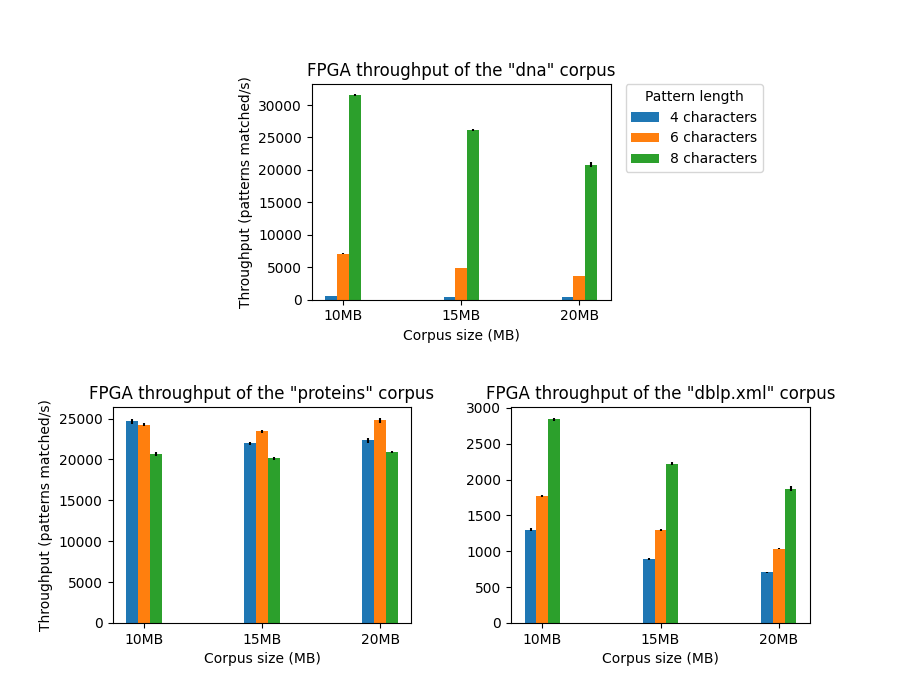
\includegraphics[width=1.0\textwidth]{figures/throughput_fpga.png}
\caption{Average throughput over 5 runs for the FPGA reference application. The \textit{dna}, \textit{proteins} and \textit{dblp.xml} corpora are showns for different pattern lengths and corpus sizes. Note that the y-axis has a different scale for each figure.}
\label{fig:throughput_fpga}
\end{figure}

Figure \ref{fig:speedup_fpga} shows the speedup of the FPGA reference applciation compared to the reference CPU application.
We see that in all cases that the FPGA performs 13 to 20 times worse than the CPU version.

\begin{figure}[H]
\centering
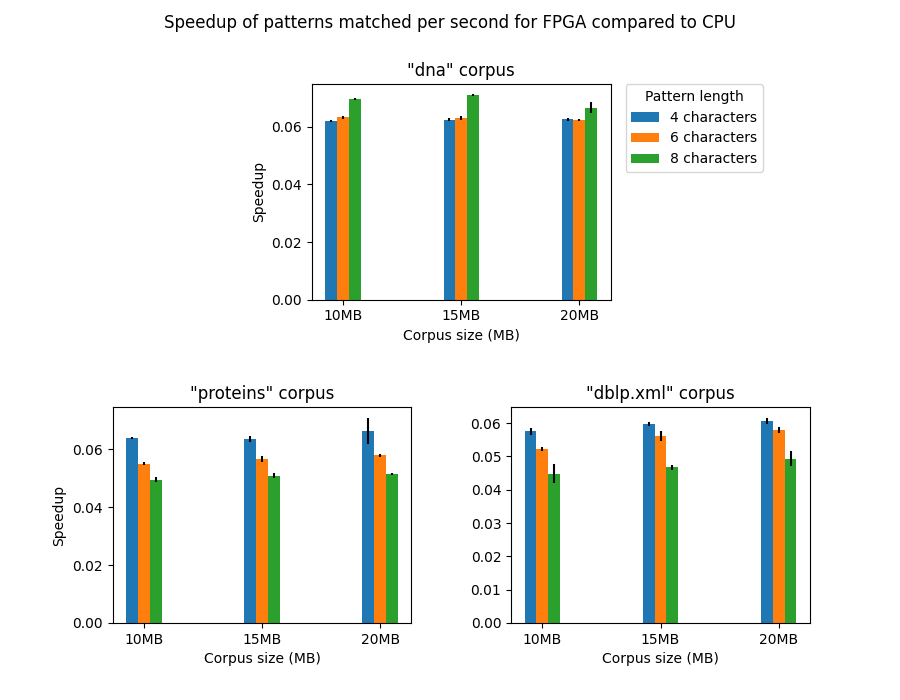
\includegraphics[width=1.0\textwidth]{figures/speedup_fpga.png}
\caption{Speedup in terms of patterns matches per second of the FPGA reference application compared to the CPU reference application for different corpora, corpus sizes and pattern lengths.}
\label{fig:speedup_fpga}
\end{figure}

We recognize that the FPGA runs on a much lower clock frequency than the CPU: 300 MHz to 3400 MHz respectively.
Therefore, it is also useful to look into the throughput in terms of patterns matches per clock cycle, instead of per second.
Figure \ref{fig:speedup_cycles_fpga} shows a comparison between the FPGA and CPU reference application in terms of pattterns matches per clock cycle.
With this metric we see that the FPGA version is only 0.5 to 0.8 times slower than the CPU.

\begin{figure}[H]
\centering
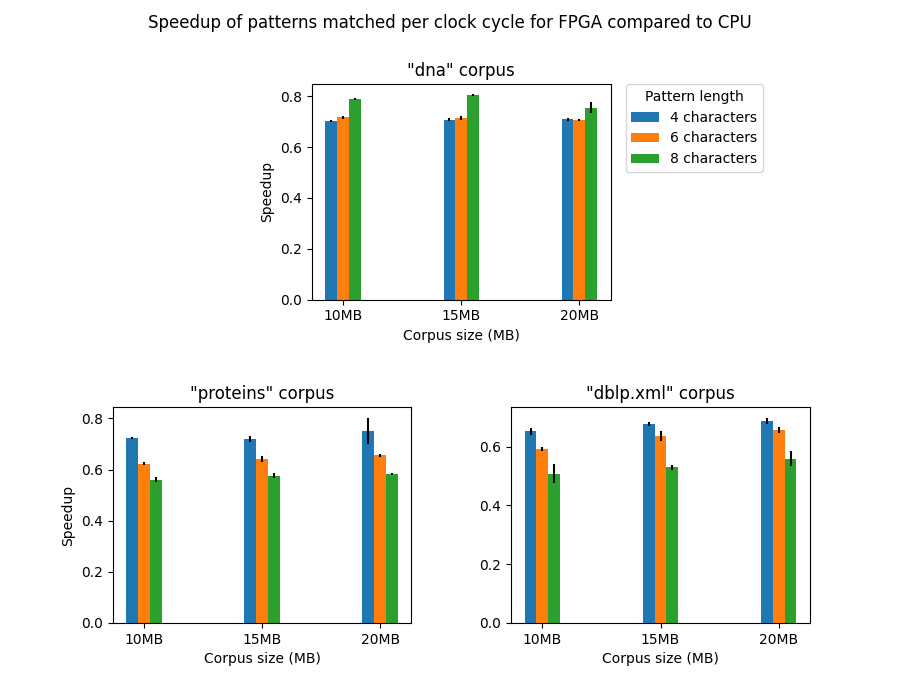
\includegraphics[width=1.0\textwidth]{figures/speedup_cycles_fpga.png}
\caption{Speedup in terms of patterns matches per clock cycle of the FPGA reference application compared to the CPU reference application for different corpora, corpus sizes and pattern lengths.}
\label{fig:speedup_cycles_fpga}
\end{figure}
